\documentclass{article}
\usepackage{pgfplots}
\usepackage{tikz}
\usepackage{chngcntr}
\counterwithin*{equation}{section}
\counterwithin*{equation}{subsection}

\title{Clairaut Equations and Singular Solutions}
\author{Tyler Yang}
\date{March 2024}

\begin{document}

\maketitle

\section{Problem Statement}
An equation of the form
\begin{equation}
y = x \frac{dy}{dx} + f(\frac{dy}{dx})
\end{equation}

\noindent where the continuously differentiable function \textit{f(t)} is evaluated at \textit{ t = dy/dx}, is called a \textbf{Clairaut equation}. Interest in these equations is due to the fact that a Clairaut equation has a one-parameter family of solutions that consist of \textit{straight lines}. Further, the \textbf{envelope} of this family---that is, the curve whose tangent lines are given by the family---is also a solution to the Clairaut equation and is called the \textbf{singular solution}.\newline

\noindent To solve a Clairaut equation:\newline

\noindent\textbf{(a)} Differentiate the Clairaut equation with respect to x and simply to show that
\begin{equation}
[x + f'(\frac{dy}{dx})] \frac{d^2y}{dx^2} = 0,
\end{equation}
where 
\begin{equation}
\end{equation}
\textit{\[f'(t) = \frac{d}{dt}f(t).\]}

\noindent\textbf{(b)} From equation (2), you can conclude that dy/dx = c or f'(dy/dx) = -x. Assume that dy/dx = c and substitute back into equation (1) to obtain the family of \textit{straight line solutions}

\begin{equation}
y = cx + f(c).
\end{equation}

\noindent\textbf{(c)} Show that another solution to equation (1) is given parametrically by 

\begin{equation}
x = -f'(p),
\end{equation}
\begin{equation}
y = f(p)  - pf'(p)
\end{equation}
where the parameter \textit{p = dy/dx}. This solution is the \textit{singular solution}.

\noindent\textbf{(d)} Use the above method to find the family of straight-line solutions and the singular solution to the equation
\begin{equation}
y = x(\frac{dy}{dx}) + 2(\frac{dy}{dx})^2
\end{equation}

\noindent Here $\mathit{f(t) = 2t^2.}$ Sketch several of the straight-line solutions along with the singular solution on the same coordinate system. Observe that the straight-line solutions are all tangent to the singular solution.\newline

\noindent\textbf{(e)} Repeat part (d) for the equation
\begin{equation}
x (\frac{dy}{dx})^3 - y(\frac{dy}{dx}) + 2 = 0
\end{equation}

\section{My Work}
\subsection{Part (a)}
\begin{equation}
y = x(\frac{dy}{dx}) + f(\frac{dy}{dx})
\end{equation}
Using Product Rule and Chain Rule for Derivatives:
\begin{equation}
\frac{d}{dx}(y) = \frac{dy}{dx} = \frac{d}{dx}[x(\frac{dy}{dx}) + f(\frac{dy}{dx})]
\end{equation}
\begin{equation}
\frac{dy}{dx} = [\frac{d}{dx}(x)][\frac{dy}{dx}] + [x][\frac{d}{dx}(\frac{dy}{dx})] + \frac{d}{dx}[f(\frac{dy}{dx})]
\end{equation}
Compute the derivatives and apply the rules to get
\begin{equation}
\frac{dy}{dx} = [1][\frac{dy}{dx}] + [x][\frac{d^2y}{dx^2}] + [f'(\frac{dy}{dx})][\frac{d^2y}{dx^2}]
\end{equation}
Notice that \textit{dy/dx} cancels out on the left and right sides.
\begin{equation}
0 = [x][\frac{d^2y}{dx^2}] + [f'(\frac{dy}{dx})][\frac{d^2y}{dx^2}]
\end{equation}
Rearrange the equation.
\begin{equation}
0 = \frac{d^2y}{dx^2}[x + f'(\frac{dy}{dx})]
\end{equation}
This is the same as equation (2) from the Problem Statement, Part (a).

\subsection{Part (b)}
Assume that \textit{dy/dx = c.} We make this assumption because in order for our solution from part (a) to be true, either  
\begin{equation}
\frac{d^2y}{dx^2} = 0,
\end{equation}
which means \textit{dy/dx = c}, where c is some constant, or
\begin{equation}
[x + f'(\frac{dy}{dx})] = 0
\end{equation}
For part (b), we assume the former condition is true. Substitute \textit{dy/dx = c.} back into equation (1) from the Problem Statement, Part (a).
\begin{equation}
y = x \frac{dy}{dx} + f(\frac{dy}{dx}) = cx + f(c)
\end{equation}
This is the family of straight-line solutions to the Clairaut equation.

\subsection{Part (c)}
Now, we deal with the latter condition:
\begin{equation}
[x + f'(\frac{dy}{dx})] = 0,
\end{equation}
which means 
\begin{equation}
x = -f'(\frac{dy}{dx})
\end{equation}
Define a new variable \textit{p = dy/dx.} Substitute \textit{p} into the previous equation to get
\begin{equation}
x = -f'(p)
\end{equation}
Substitute \textit{p} into the original Clairaut equation to get
\begin{equation}
y = x \frac{dy}{dx} + f(\frac{dy}{dx}) = [-f'(p)][p] + f(p) = f(p) - pf'(p)
\end{equation}
This is the singular solution to the Clairaut equation.


\subsection{Part (d)}
Now, we finally get to solve an example problem!
\begin{equation}
y = x \frac{dy}{dx} + 2(\frac{dy}{dx})^2
\end{equation}
\begin{equation}
\frac{d}{dx}(y) = \frac{dy}{dx} = (1)(\frac{dy}{dx}) + (\frac{d^2y}{dx^2})(x) + 4(\frac{dy}{dx})(\frac{d^2y}{dx^2})
\end{equation}
\begin{equation}
\frac{dy}{dx} = \frac{dy}{dx} + \frac{d^2y}{dx^2}[x + 4(\frac{dy}{dx})]
\end{equation}
\begin{equation}
0 = \frac{d^2y}{dx^2}[x + 4(\frac{dy}{dx})]
\end{equation}
Solve for the singular solution:
\begin{equation}
x = -4(\frac{dy}{dx})
\end{equation}
Note that this is actually a separable differential equation!
\begin{equation}
-\frac{x}{4} dx = dy
\end{equation}
\begin{equation}
y = -\frac{x^2}{8} + C
\end{equation}
But let's solve it the parametric way too:
\begin{equation}
f(t) = 2t^2 \rightarrow f'(t) = 4t
\end{equation}
\begin{equation}
y = f(p) - pf'(p) = 2(\frac{dy}{dx})^2 - (\frac{dy}{dx})(4)(\frac{dy}{dx}) = -2(\frac{dy}{dx})^2
\end{equation}
If we parameterize \textit{p} to a more conventional variable like \textit{t}, what we have in a simple 2-dimensional parametric equation:
\begin{equation}
x = -4t, y= -2t^2
\end{equation}
Which can be defined explicitly as:
\begin{equation}
y = -\frac{x^2}{8}.
\end{equation}
Note that this is the same as solving for the solution through separating and integrating, with constant C set to zero. Nonetheless, let's move onto the straight line solutions:
\begin{equation}
\frac{dy}{dx} = c
\end{equation}
\begin{equation}
y = cx + 2(c)^2
\end{equation}
\begin{center}
\begin{tabular}{| c | c |}
\hline
c & y \\
\hline
 1 & x + 2  \\
 \hline
 2 & 2x + 8  \\
 \hline
 -1 & -x + 2  \\
 \hline
 -2 &  -2x + 8 \\
\hline
\end{tabular}
\end{center}

\subsubsection{Graphing the solutions}
\begin{center}
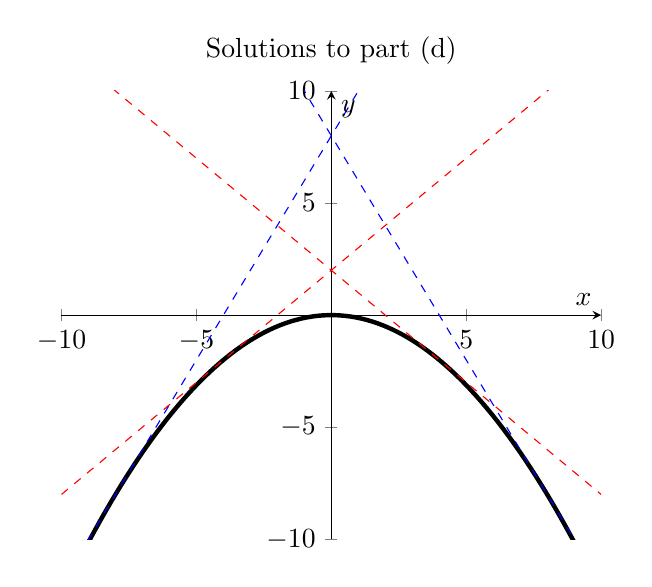
\begin{tikzpicture}
\begin{axis}[xmin=-10, xmax=10, ymin=-10, ymax=10, 
axis lines = middle, 
xlabel=$x$, 
ylabel=$y$, 
title = {Solutions to part (d)}
]
\addplot[color = black, samples = 100, domain=-10:10, ultra thick]{-x^2/8};
\addplot[color = red, samples = 10, domain=-10:10, dashed]{x+2};
\addplot[color = red, samples = 10, domain=-10:10, dashed]{-x+2};
\addplot[color = blue, samples = 10, domain=-10:10, dashed]{2*x+8};
\addplot[color = blue, samples = 10, domain=-10:10, dashed]{-2*x+8};
\end{axis}
\end{tikzpicture}
\end{center}

\subsubsection{Final Answer}
The Clairaut equation
\begin{equation}
y = x \frac{dy}{dx} + 2(\frac{dy}{dx})^2
\end{equation}
has a single solution
\begin{equation}
y = -\frac{x^2}{8}
\end{equation}
which envelopes the family of straight-line solutions given by
\begin{equation}
y = cx + 2c^2
\end{equation}

\subsection{Part (e)}
Now we will solve another Clairaut equation:
\begin{equation}
x(\frac{dy}{dx})^3 - y(\frac{dy}{dx})^2 + 2 = 0.
\end{equation}
Rearrange to get it in the form of a Clairaut equation:
\begin{equation}
y(\frac{dy}{dx})^2 = x(\frac{dy}{dx})^3 + 2
\end{equation}
\begin{equation}
y = x(\frac{dy}{dx}) + 2(\frac{dy}{dx})^{-2}
\end{equation}
Take the derivative of y:
\begin{equation}
\frac{d}{dx}(y) = \frac{dy}{dx} = [1][\frac{dy}{dx}] + [x][\frac{d^2y}{dx^2}] -4(\frac{dy}{dx})^{-3}(\frac{d^2y}{dx^2})
\end{equation}
\begin{equation}
0 = \frac{d^2y}{dx^2}[x-4(\frac{dy}{dx})^{-3}]
\end{equation}
Solve for singular solution:
\begin{equation}
x = -4(\frac{dy}{dx})^{-3}
\end{equation}
\begin{equation}
p = \frac{dy}{dx}, f(t) = \frac{2}{t^2}
\end{equation}
\begin{equation}
y = f(p) - pf'(p)
\end{equation}
\begin{equation}
y = 2(\frac{dy}{dx})^{-2} - \frac{dy}{dx}[-4(\frac{dy}{dx})^{-3}]
\end{equation}
\begin{equation}
y = 6(\frac{dy}{dx})^{-2}
\end{equation}
Reparametrizing \textit{dy/dx} with \textit{t}, This leaves us with two parametric equations:
\begin{equation}
x = 4t^{-3}, y = 6t^{-2}
\end{equation}
Rewrite \textit{y} explicitly in terms of \textit{x}:
\begin{equation}
y = 6(\frac{x}{4})^{2/3}
\end{equation}
Now we solve for the straight-line family of solutions:
\begin{equation}
\frac{d^2y}{dx^2} = 0 \rightarrow \frac{dy}{dx} = c
\end{equation}
\begin{equation}
y = cx + 2c^{-2}
\end{equation}
\begin{center}
\begin{tabular}{| c | c |}
\hline
c & y \\
\hline
 1 & x + 2  \\
 \hline
 2 & 2x + 1/2 \\
 \hline
 -1 & -x + 2  \\
 \hline
 -2 &  -2x + 1/2 \\
\hline
\end{tabular}
\end{center}

\subsubsection{Graphing the solutions}
\begin{center}
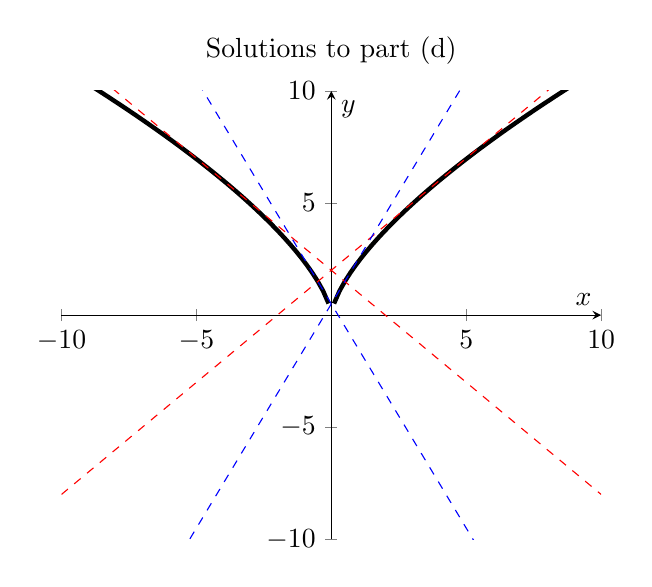
\begin{tikzpicture}
\begin{axis}[xmin=-10, xmax=10, ymin=-10, ymax=10, 
axis lines = middle, 
xlabel=$x$, 
ylabel=$y$, 
title = {Solutions to part (d)}
]
\addplot[color = black, samples = 100, domain=-10:10, ultra thick]{6*(x/4)^(2/3)};
\addplot[color = black, samples = 100, domain=-10:10, ultra thick]{6*(-x/4)^(2/3)};
\addplot[color = red, samples = 10, domain=-10:10, dashed]{x+2};
\addplot[color = red, samples = 10, domain=-10:10, dashed]{-x+2};
\addplot[color = blue, samples = 10, domain=-10:10, dashed]{2*x+1/2};
\addplot[color = blue, samples = 10, domain=-10:10, dashed]{-2*x+1/2};
\end{axis}
\end{tikzpicture}
\end{center}

\subsubsection{Final Answer}
The Clairaut equation
\begin{equation}
x(\frac{dy}{dx})^3 - y(\frac{dy}{dx})^2 + 2 = 0.
\end{equation}
has a single solution
\begin{equation}
y = 6(\frac{x}{4})^{2/3}
\end{equation}
which envelopes the family of straight-line solutions given by
\begin{equation}
y = cx + 2c^{-2}
\end{equation}


\end{document}
\begin{equation}
\end{equation}